\section{GRASS Integration}\label{sec:grass}\index{GRASS}

% when the revision of a section has been finalized, 
% comment out the following line:
\updatedisclaimer

The GRASS~\cite{GRASSweb} plugin provides access to GRASS from within QGIS. 
This includes the ability to view, edit, and create data, as well as perform 
analysis using the GRASS geoprocessing modules.

In this chapter we'll introduce the plugin and some of the ways you can use 
it to work with GRASS data. The following features are provided with the GRASS 
plugin:
 
\begin{itemize}
\item \toolbtntwo{grass_open_mapset}{Open mapset}
\item \toolbtntwo{grass_new_mapset}{New mapset}
\item \toolbtntwo{grass_close_mapset}{Close mapset}
\item \toolbtntwo{grass_add_vector}{Add GRASS vector layer}
\item \toolbtntwo{grass_add_raster}{Add GRASS raster layer}
\item \toolbtntwo{grass_new_vector_layer}{Create new GRASS vector}
\item \toolbtntwo{grass_edit}{Edit GRASS vector layer}
\item \toolbtntwo{grass_tools}{Open GRASS tools}
%\item \toolbtntwo{grass_shell}{Open GRASS Shell}
\item \toolbtntwo{grass_region}{Display current GRASS region} 
\item \toolbtntwo{grass_region_edit}{Edit current GRASS region}
\end{itemize}

\subsection{Starting QGIS with GRASS}\label{sec:starting_grass}
\index{GRASS!starting QGIS}

To use GRASS features from within QGIS, you must select and load the GRASS
plugin with the Plugin Manager clicking on \mainmenuopt{Plugins} >
\mainmenuopt{Manage Plugins}. Inside the QGIS Plugin Manager you need to
select \dropmenuopt{GRASS} and click \button{OK}. A new toolbar with the 10
buttons described above will appear on the user interface and you can
immediately start loading layers of an existing GRASS dataset (location)
using the appropriate toolbar buttons for vector and raster data (see Section
\ref{sec:load_grassdata}). Or you can create a new GRASS \filename{location}
with QGIS (see Section \ref{sec:create_loc}).

\subsection{Loading GRASS Data}\label{sec:load_grassdata}\index{GRASS!loading
data}

With the GRASS plugin, you can load vector or raster layers using the
appropriate button on the toolbar. As an example we use the QGIS alaska
dataset. It includes a small sample GRASS location with 3 vector layers and 1
raster elevation map (see Section \ref{label_sampledata}).

\begin{enumerate}
  \item Create a new folder \filename{grassdata}, download the QGIS alaska
  dataset \filename{qgis\_data\_2008\_09\_15.zip} from
  \url{http://download.osgeo.org/qgis/data/} and unzip the file into
  \filename{grassdata}. 
  \item Start QGIS.
  \item If not already done in a previous QGIS session, load the GRASS plugin
  clicking on \mainmenuopt{Plugins} > \mainmenuopt{Manage Plugins} and
  selecting \dropmenuopt{GRASS}. The GRASS toolbar appears on the user
  interface.
  \item In the GRASS toolbar, click on the \toolbtntwo{grass_open_mapset}{Open
  mapset} icon to bring up the mapset wizard.
  \item For \filename{Gisdbase} browse and select or enter the path to the
  newly created folder \filename{grassdata}.
  \item You should now be able to select the location \filename{alaska}
  and the mapset \filename{demo}. 
  \item Click \button{OK}. Notice that some of the tools in the GRASS toolbar
  that were disabled are now enabled.
  \item Click on \toolbtntwo{grass_add_raster}{Add GRASS raster layer},
  choose the map name \filename{gtopo30} and click \button{OK}. The elevation
  layer will be visualized. 
  \item Click on \toolbtntwo{grass_add_vector}{Add GRASS vector layer},
  choose the map name \filename{alaska} and click \button{OK}. Now the alaska
  boundary vector layer will be overlayed on top of the geology map. You can
  now adapt the layer properties as described in chapter \ref{sec:vectorprops},
  e.g. change opacity, fill and outline color.
  \item Also load the other two vector layers \filename{rivers} and
  \filename{airports} and adapt their properties.
\end{enumerate}

As you see, it is very simple to load GRASS raster and vector layers in QGIS. 
See following sections for editing GRASS data and creating new locations.
More sample GRASS locations are available at the GRASS website at
\url{http://grass.osgeo.org/download/data.php}.

\begin{Tip}\caption{\textsc{GRASS Data Loading}}
\qgistip{If you have problems loading data or QGIS terminates abnormally,
check to make sure you have loaded the GRASS plugin properly as described in
Section \ref{sec:starting_grass}.
}
\end{Tip} 

\subsection{Creating a GRASS location}\label{sec:create_loc}

In order to analyse your vector and raster layers with GRASS modules, you
must import your data into a GRASS database, calles \filename{location}. A
location represents a specific area with a specific coordinate
system.\footnote{This is not strictly true - with the GRASS modules
\filename{v.external} and \filename{r.external} you can create read-only
links to external OGR-supported data sets without importing them. But this is
not the standard way to work with GRASS.}

\begin{figure}[ht]
\begin{center}
\caption{Creating a new GRASS location in QGIS \nixcaption}\label{fig:grass_location}\smallskip
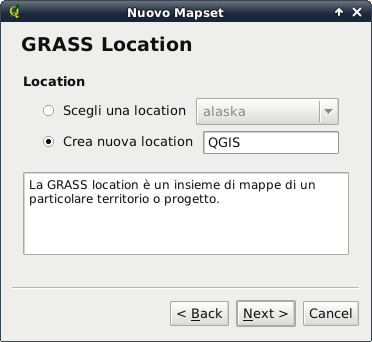
\includegraphics[clip=true]{create_grass_location}
\end{center}  
\end{figure}

As an an example you find below the instructions how the sample GRASS
location \filename{alaska}, which is projected in Albers Equal Area
projection with unit meter was created for the QGIS sample dataset. This
sample GRASS location \filename{alaska} will be used for all examples and
exercises in the following GRASS GIS related chapters, so it is useful to
download and install the dataset on your computer \ref{label_sampledata}).

\begin{enumerate}
  \item Start QGIS and make sure the GRASS plugin is loaded
  \item Visualize the \filename{alaska.shp} shapefile (see Section
  \ref{sec:load_shapefile}) from the QGIS alaska dataset.
  \item In the GRASS toolbar, click on the \toolbtntwo{grass_open_mapset}{Open
    mapset} icon to bring up the mapset wizard.
  \item Each location is stored in a directory usually named
  \filename{grassdata}. Select an existing GRASS database folder, usually
  named \filename{grassdata} or create one for storing the new location.
  \item Click \button{Next}. 
  \item We can use this wizard to create a new mapset within an existing 
  location or to create a new location altogether. Click on the radio button
  \radiobuttonon{Create new location} (see Figure \ref{fig:grass_location}).
  \item Enter a name for the location - we used alaska
  \item Click \button{Next} 
  \item Define the projection by clicking on the radio button
  \radiobuttonon{Projection} to enable the projection list 
  \item We are using Albers Equal Area Alaska (meters) projection. Since we
  happen to know that it is represented by the EPSG ID 5000, we enter it in
  the search box. (If you want to repeat this process for another location
  and projection and haven't memorized the EPSG ID, click on the
  \toolbtntwo{mIconProjectionEnabled}{projector} icon in the lower right-hand
  corner of the status bar (see Section \ref{label_projstart}).
  \item Click \button{Find} to select the projection
  \item Click \button{Next} 
  \item To define the default region, we have to enter the boundaries in the
  north, south, east, and west direction. Here we simply click on the button
  \button{Set current QGIS extent}, to apply the extend of the loaded layer
  \filename{alaska.shp} as the GRASS default region extend.
  \item Click \button{Next} 
  \item We need to define a mapset within our new location. You can name it
  whatever you like - we used demo. Later you will see, that another standard
  mapset named \filename{PERMANENT} was automatically created, too. It has to
  exist and includes important definitions and configurations for the
  location.
  \item Check out the summary to make sure it's correct and click
  \button{Finish} 
  \item The new location \filename{alaska} and two mapsets \filename{demo}
  and \filename{PERMANENT} are created. The currently opened working set is
  mapset \filename{demo}, as you defined.
  \item Notice that some of the tools in the GRASS toolbar that were 
  disabled are now enabled for us to use.
\end{enumerate}

If that seemed like a lot of steps, it's really not all that bad and a very 
quick way to create a location. The location \filename{alaska} would now be
ready for data import. But as you know, we already did these steps for you and
also imported some data into the sample GRASS location \filename{alaska}
included in the QGIS alaska dataset. So you can move on to the following
chapters and learn how to digitize and edit GRASS vector layer and how to
work with the GRASS Toolbox. 

\subsection{Vector Data Model}\label{label_vectmodel}\index{GRASS!vector data
model}

It is important to understand the GRASS vector data model prior to
digitizing.\index{GRASS!digitizing} In general, GRASS uses a topological
vector model.\index{GRASS!topology} This means that areas are not represented
as closed polygons, but by one or more boundaries. A boundary between two
adjacent areas is digitized only once, and it is shared by both areas.
Boundaries must be connected without gaps. An area is identified (labeled) by
the centroid of the area.

Besides boundaries and centroids, a vector map can also contain
points and lines. All these geometry elements can be mixed
in one vector and will be represented in different so called 'layers' inside
one GRASS vector map. So in GRASS a layer is not a vector or raster map but a
level inside a vector layer. This is important to distinguish carefully.
\footnote{Although it
is possible to mix geometry elements, it is unusual and even in GRASS only
used in special cases such as vector network analysis. Normally you should
prefere to store different geometry elements in different layers.}

It is possible to store more 'layers' in one vector dataset. For example,
fields, forests and lakes can be stored in one vector. Adjacent
forest and lake can share the same boundary, but they have separate attribute
tables. It is also possible to attach attributes to boundaries. For example,
the boundary between lake and forest is a road, so it can have a different 
attribute table.
 
The 'layer' of the feature is defined by 'layer' inside GRASS.
'Layer' is the number which defines if there are more than one layer inside the 
dataset, e.g. if the geometry is forest or lake.
For now, it can be only a number, in the future GRASS will also support  
names as fields in the user interface.

Attributes can be stored inside the GRASS location as DBase or SQLITE3 or in
external database tables, for example PostgreSQL, MySQL, Oracle,
etc.\index{GRASS!attribute storage}

Attributes in database tables are linked to geometry elements using
a 'category' value.\index{GRASS!attribute linkage} 'Category' (key, ID) is an
integer attached to geometry primitives, and it is used as the link to one
key column in the database table.

\begin{Tip}\caption{\textsc{Learning the GRASS Vector Model}}
\qgistip{
The best way to learn the GRASS vector model and its capabilities is to 
download one of the many GRASS tutorials where the vector model is described
more deeply. See \url{http://grass.osgeo.org/gdp/manuals.php} for more
information, books and tutorials in several languages.
}
\end{Tip} 

\subsection{Digitizing and Editing Tools}\index{GRASS!digitizing tools}
\label{grass_digitising}

The digitizing tools for GRASS vector layers are accessed using the
\toolbtntwo{grass_edit}{Edit GRASS vector layer} icon on the toolbar. Make sure
you have loaded a GRASS vector and it is the selected layer in the legend before
clicking on the edit tool. If you want to create a new GRASS vector layer, 
you need to click on the \toolbtntwo{grass_new_vector_layer}{Create new GRASS
vector} icon. Figure \ref{fig:grass_digitizing} shows the GRASS edit dialog
that is displayed when you click on the edit tool. The tools and settings are
discussed in the following sections.

\subsubsection{Toolbar}\label{label_grasstoolbar}

In Figure \ref{fig:grass_digitizing_toolbar} you see the GRASS digitizing
toolbar icons provided by the GRASS plugin. Table \ref{tab:grass_tools}
explains the available functionalities.

\begin{figure}[h]
   \begin{center}
   \caption{GRASS Digitizing Toolbar \nixcaption}\label{fig:grass_digitizing_toolbar} 
   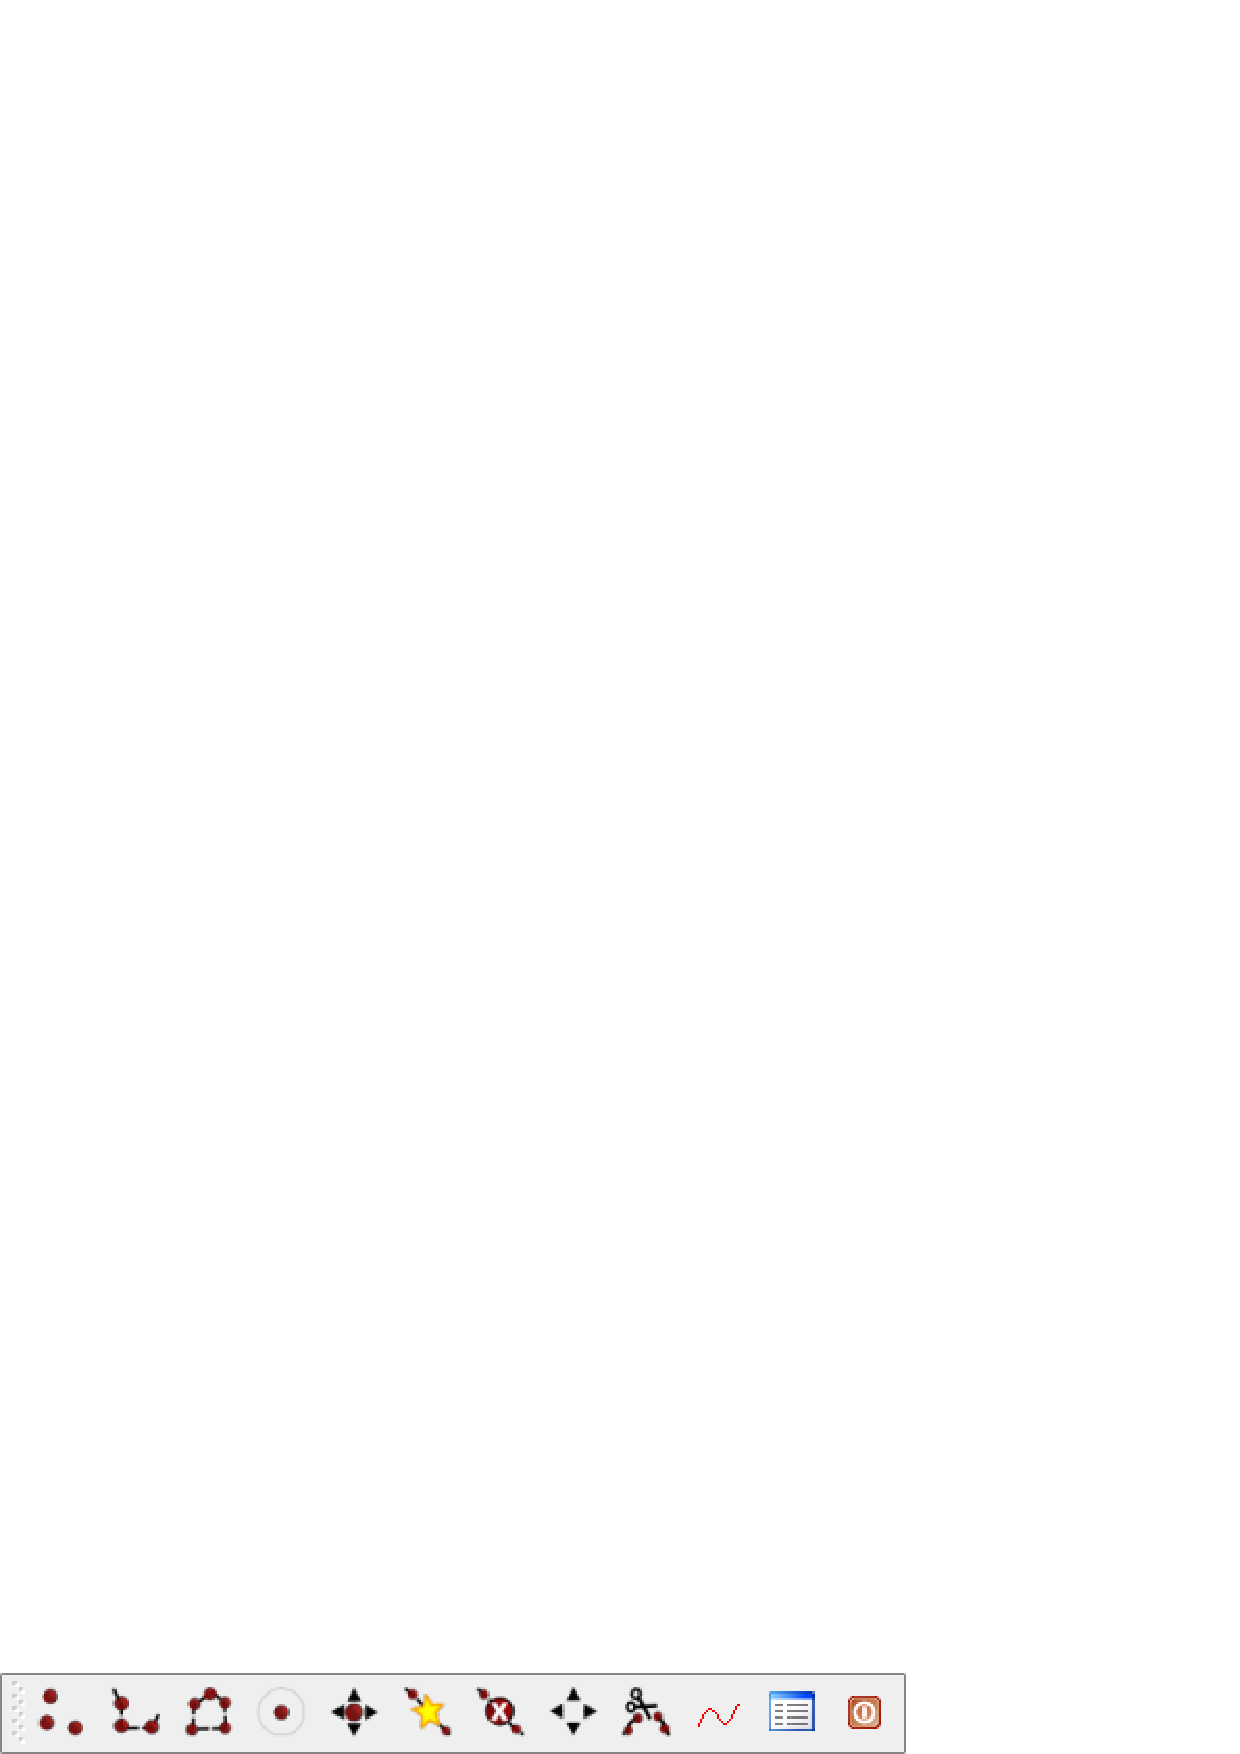
\includegraphics[clip=true,width=12cm]{grass_digitizing_toolbar}
\end{center}  
\end{figure}

\begin{table}[h]\index{GRASS!digitizing tools}
\centering
\caption{GRASS Digitizing Tools}\label{tab:grass_tools}\medskip
 \begin{tabular}{|l|l|p{5in}|}
 \hline \textbf{Icon} & \textbf{Tool} & \textbf{Purpose} \\
\hline 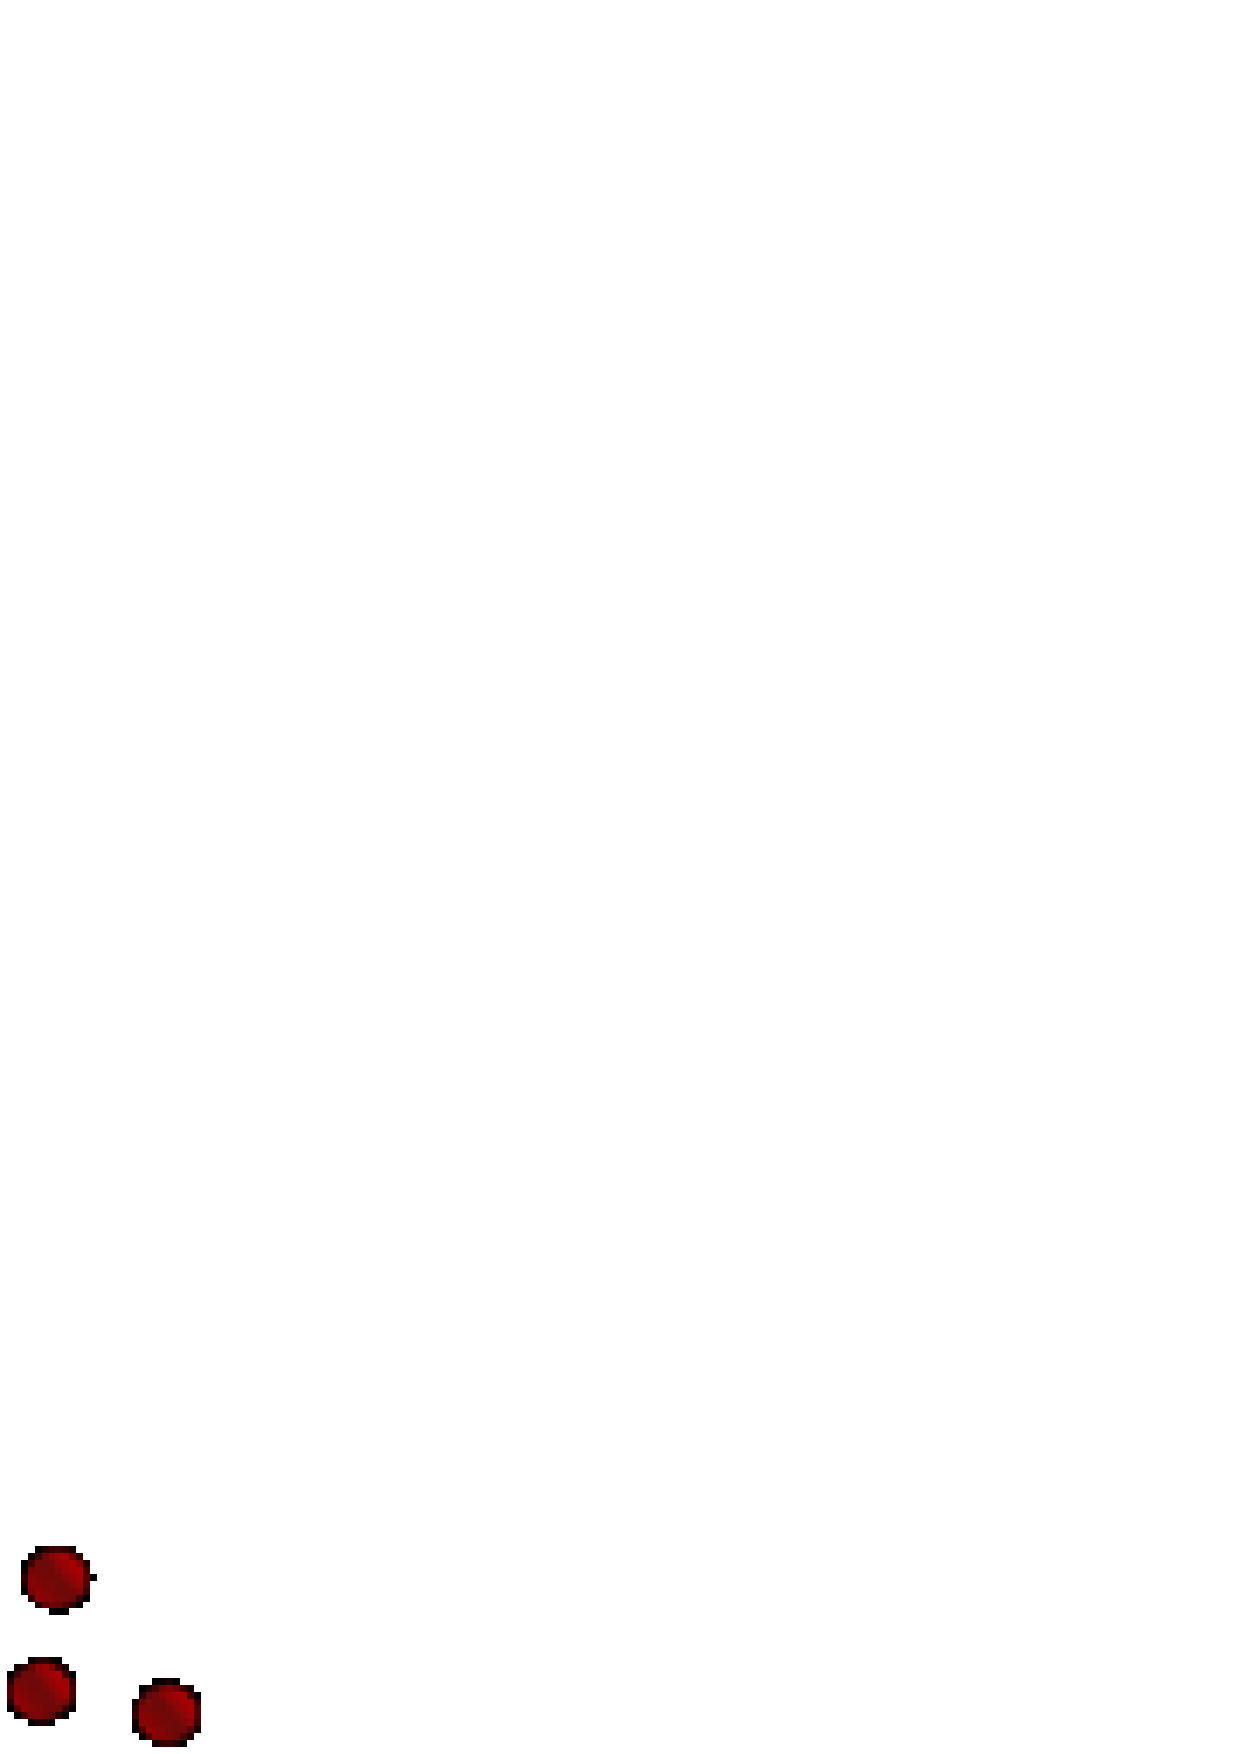
\includegraphics[width=0.7cm]{grass_new_point} & New Point & Digitize
new point \\
\hline 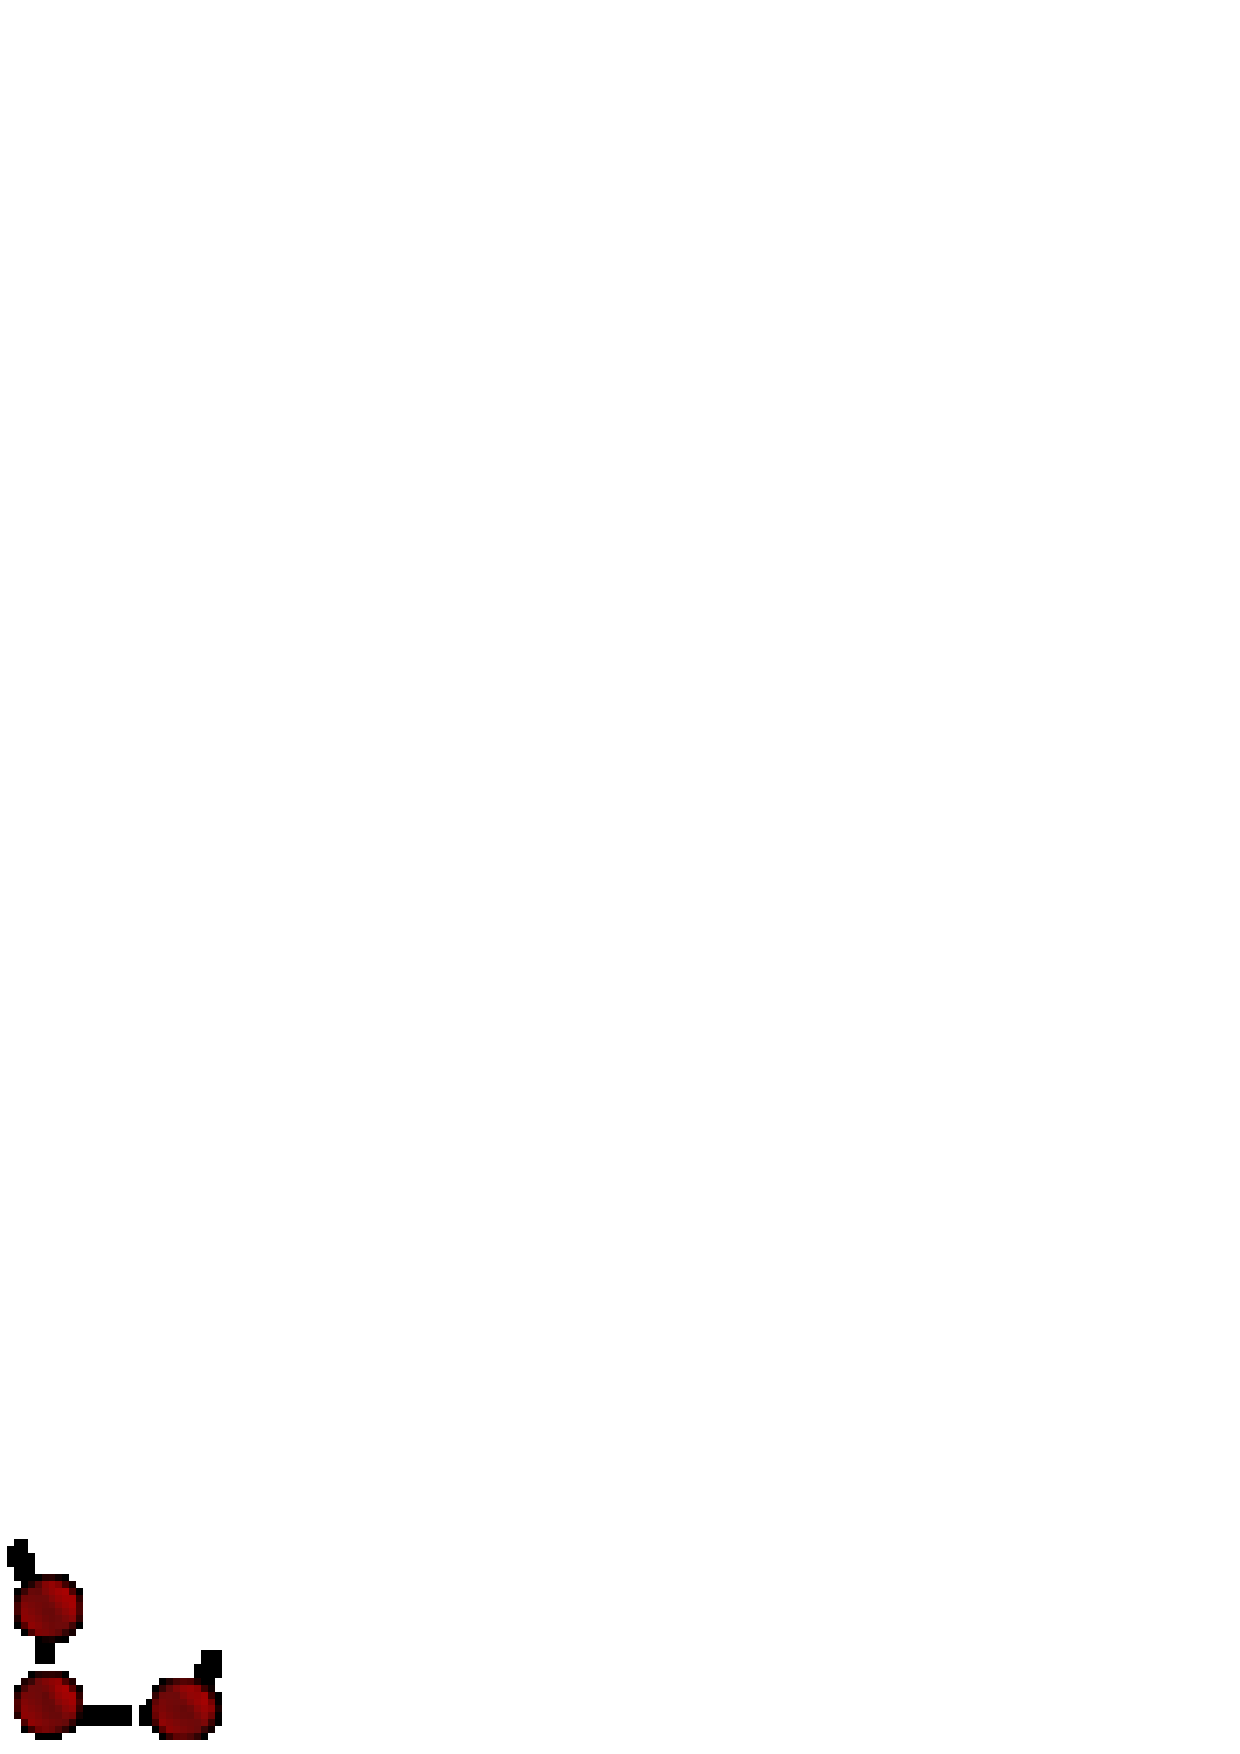
\includegraphics[width=0.7cm]{grass_new_line} & New Line & Digitize
new line (finish by selecting new tool) \\
\hline 
\includegraphics[width=0.7cm]{grass_new_boundary} & New Boundary &
Digitize new boundary (finish by selecting new tool)\\
\hline 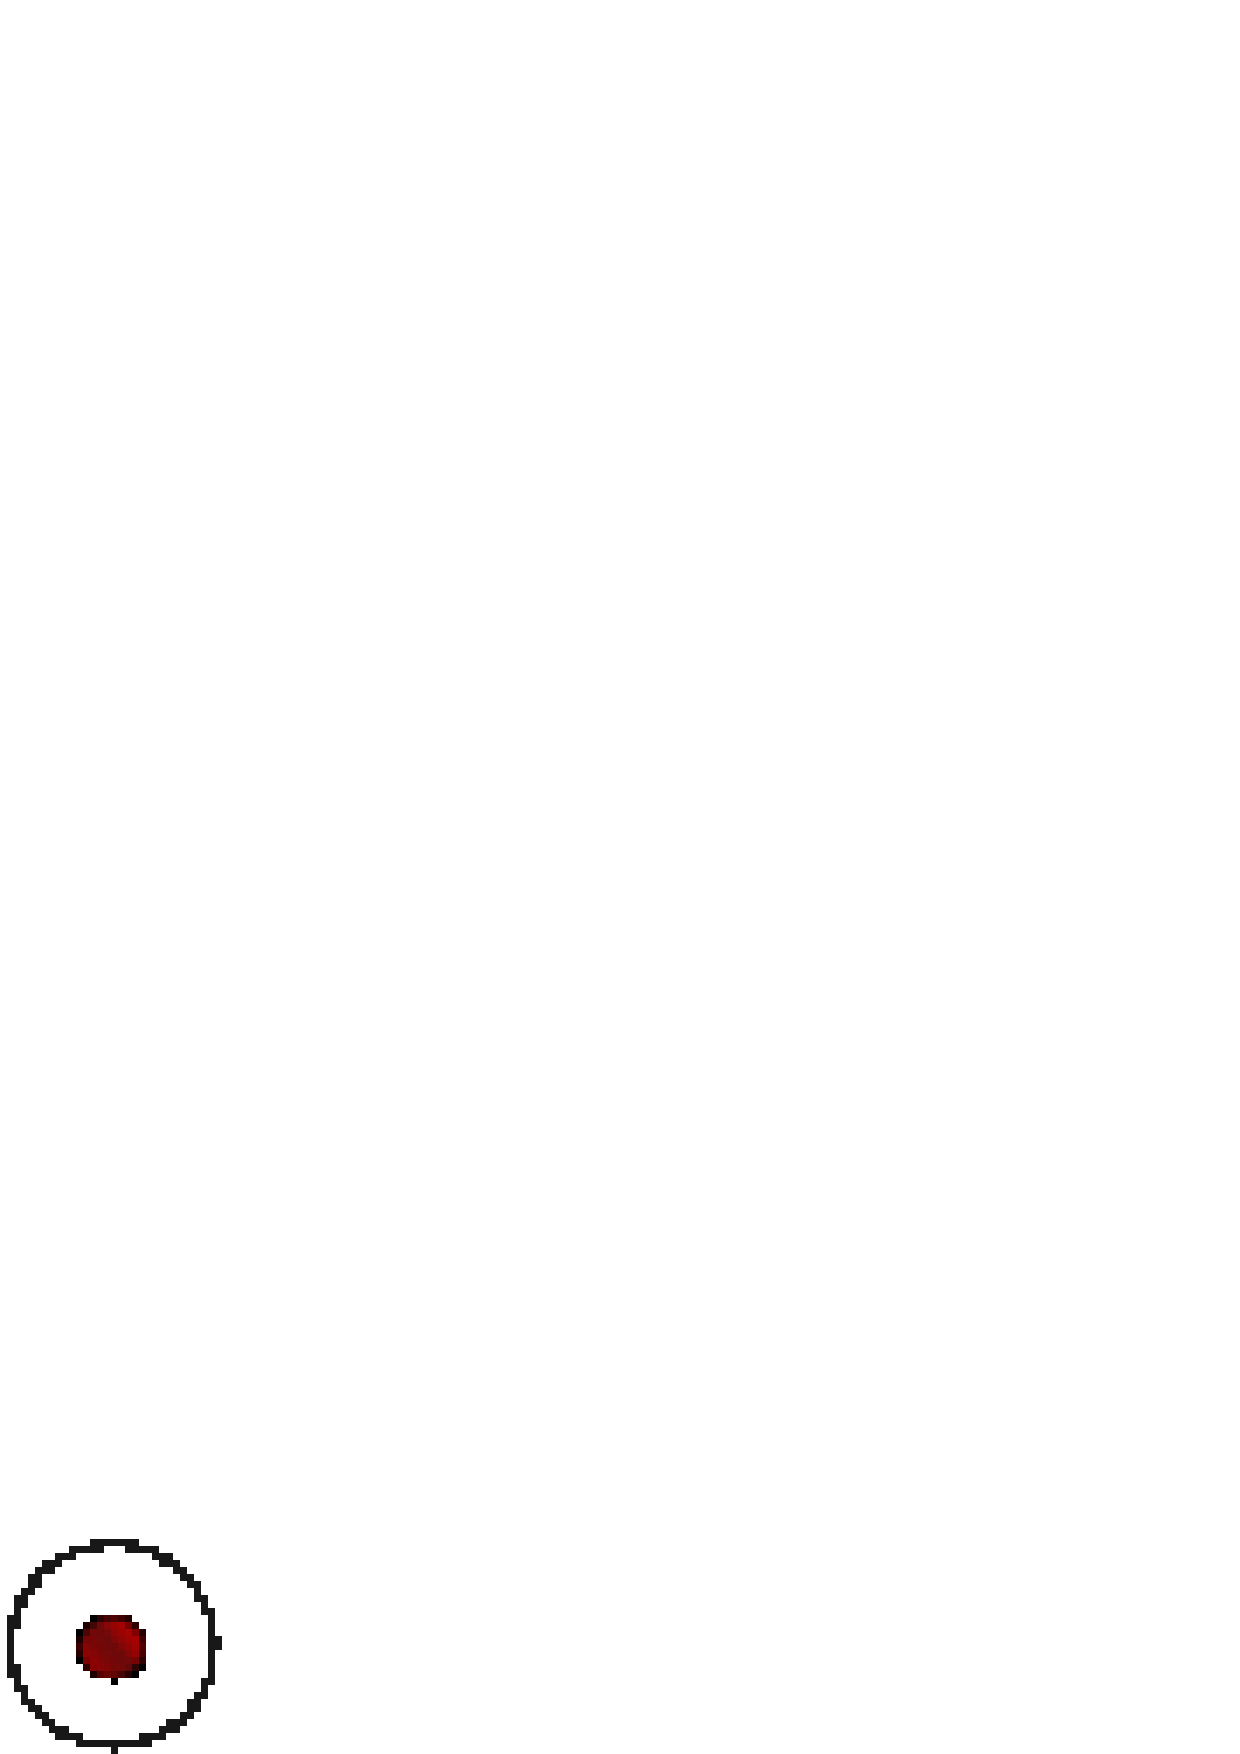
\includegraphics[width=0.7cm]{grass_new_centroid} & New Centroid &
Digitize new centroid (label existing area)\\
\hline 
\includegraphics[width=0.7cm]{grass_move_vertex} & Move vertex & Move
one vertex of existing line or boundary and identify new position\\
\hline 
\includegraphics[width=0.7cm]{grass_add_vertex} & Add vertex & Add a
new vertex to existing line\\
\hline 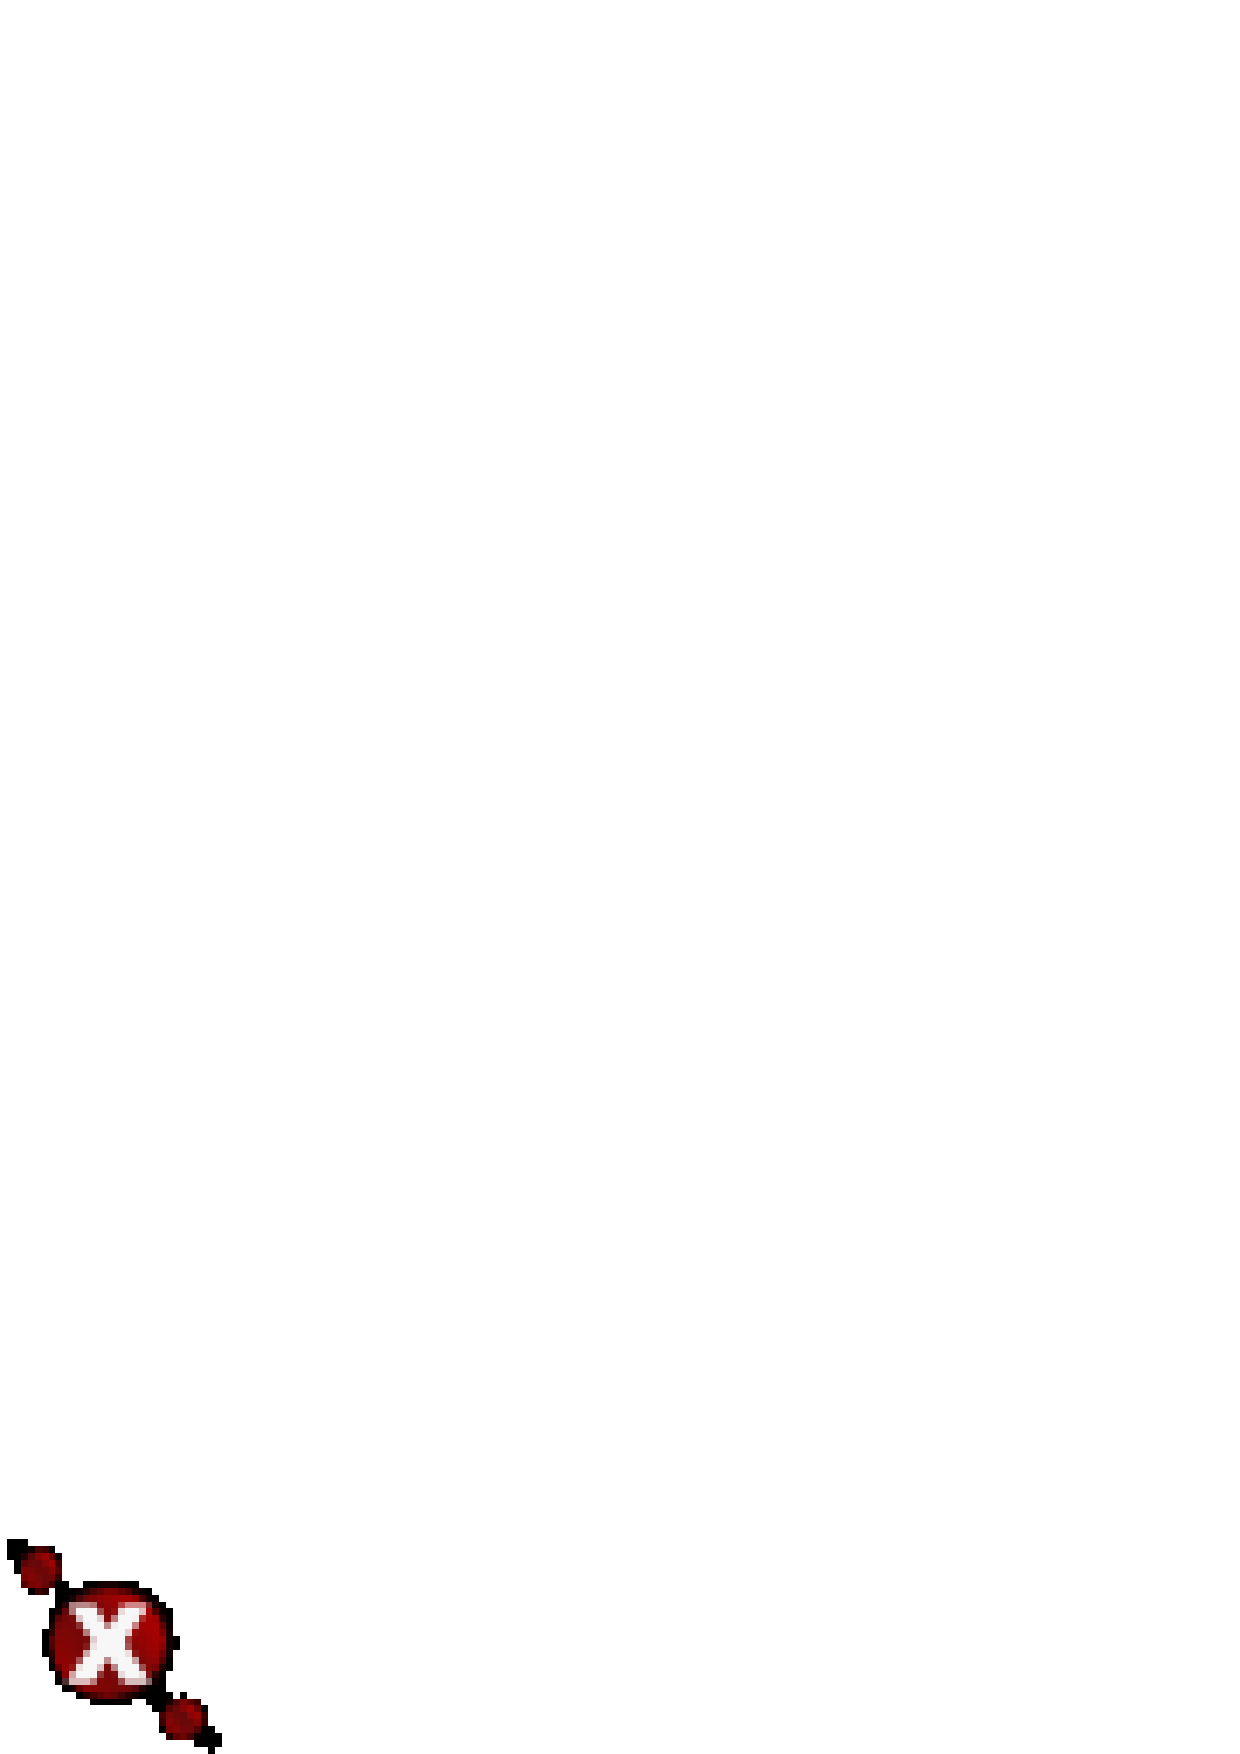
\includegraphics[width=0.7cm]{grass_delete_vertex} & Delete vertex &
Delete vertex from existing line (confirm selected vertex by another click)\\
\hline 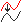
\includegraphics[width=0.7cm]{grass_move_line} & Move element & Move
selected boundary, line, point or centroid and click on new position\\
\hline 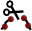
\includegraphics[width=0.7cm]{grass_split_line} & Split line & Split
an existing line to 2 parts\\
\hline 
\includegraphics[width=0.7cm]{grass_delete_line} & Delete element &
Delete existing boundary, line, point or centroid (confirm selected element by
another click)\\
\hline 
\includegraphics[width=0.7cm]{grass_edit_attributes} & Edit attributes
& Edit attributes of selected element (note that one element can represent
more features, see above)\\
\hline 
\includegraphics[width=0.7cm]{grass_close_edit} & Close & Close
digitizing session and save current status (rebuilds topology afterwards)\\
\hline
\end{tabular}
\end{table}

\subsubsection{Category Tab}\index{GRASS!category settings}

The \tab{Category} tab allows you to set the way in which the category will
be assigned to each new feature and/or assign a category to a feature.

\begin{figure}[h]
 \begin{center}
  \caption{GRASS Digitizing Category Tab \nixcaption}\label{fig:grass_digitizing_category}
  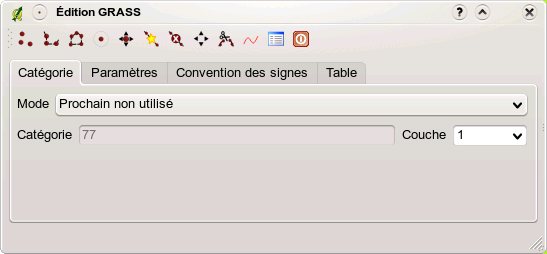
\includegraphics[clip=true,width=10cm]{grass_digitizing_category}
 \end{center}
\end{figure}

\begin{itemize}
\item \textbf{Mode}: what category value shall be applied to geometry element
\begin{itemize}
\item Next not used - apply next not yet used category value to geometry
element
\item Manual entry - manually define the category value for the geometry
element in the 'Category'-entry field
\item No category - Do not apply a category value to the geometry element.
This is e.g. used for area boundaries, because the category values are
connected via the centroid.
\end{itemize}
\item \textbf{Category} - A number (ID) attached to each digitized geometry
element. It is used to connect each geometry element with its attributes.
\item \textbf{Field (layer)} - Each geometry element can be connected with
several attribute tables using different GRASS geometry layers. Default layer
number is 1. 
\end{itemize}

\begin{Tip}\caption{\textsc{Creating an additional GRASS 'layer' with QGIS}}
\qgistip{If you would like to add more layers to your dataset, just add a new
number in the 'Field (layer)' entry box and press return. In the Table tab
you can create your new table connected to your new layer.
}
\end{Tip}

\subsubsection{Settings Tab}\label{label_settingtab}\index{GRASS!snapping
tolerance}

The \tab{Settings} tab allows you to set the snapping in screen pixels. The
threshold defines at what distance new points or line ends are snapped to
existing nodes. This helps prevent gaps or dangles between boundaries. The
default is set to 10 pixels.

\begin{figure}[h]
 \begin{center}
 \caption{GRASS Digitizing Settings Tab \nixcaption}\label{fig:grass_digitizing_settings}
 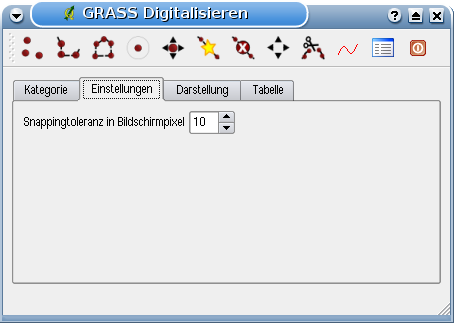
\includegraphics[clip=true,width=8cm]{grass_digitizing_settings}
 \end{center}
\end{figure}

\subsubsection{Symbology Tab}\index{GRASS!symbology settings}

The \tab{Symbology} tab allows you to view and set symbology and color
settings for various geometry types and their topological status (e.g. closed
/ opened boundary).

\begin{figure}[h]
 \begin{center}
 \caption{GRASS Digitizing Symbolog Tab \nixcaption}\label{fig:grass_digitizing_symbology}
 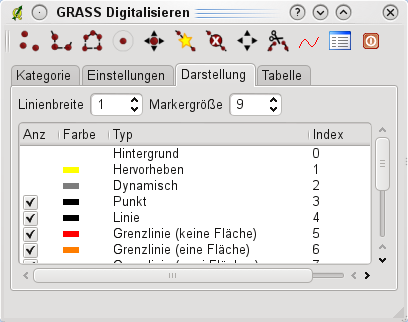
\includegraphics[clip=true,width=8cm]{grass_digitizing_symbology}
 \end{center}
\end{figure}

\subsubsection{Table Tab} \index{GRASS!table editing}

The \tab{Table} tab provides information about the database table for
a given 'layer'. Here you can add new colums to an existing attribute table,
or create a new database table for a new GRASS vector layer.

\begin{figure}[h]
 \begin{center}
 \caption{GRASS Digitizing Table Tab \nixcaption}\label{fig:grass_digitizing_table}
 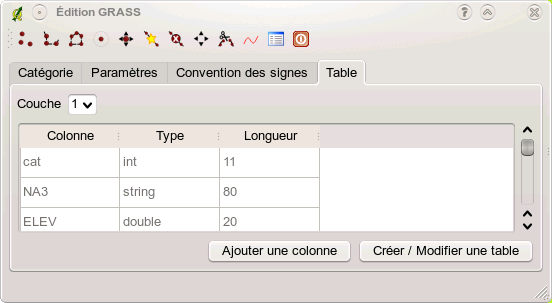
\includegraphics[clip=true,width=10cm]{grass_digitizing_table}
 \end{center}
\end{figure}

\begin{Tip}\caption{\textsc{GRASS Edit Permissions}}\index{GRASS!edit
permissions}
\qgistip{You must be the owner of the GRASS mapset you want to edit. It is
impossible to edit vectors in mapsets which are not yours, even if you have
write permissions.
}
\end{Tip} 

\subsection{Region Tool}\index{GRASS!region}

The current region (window) in GRASS is very important for all 
raster modules. All newly-created rasters have the extension and resolution
of the current region, regardless of their original region. The region is
stored in \filename{\$LOCATION/\$MAPSET/WIND} file, and it defines
north, south, east, west, number of columns, number of rows, 
horizontal and vertical spatial resolution.

It is possible to switch on/off the GRASS region in the QGIS canvas
using the \toolbtntwo{grass_region}{Display current GRASS region} button. \index{GRASS!region!display}

With the \toolbtntwo{grass_region_edit}{Edit current GRASS region} you can open a tool 
in which you can change the current region and symbology
of the GRASS region rectangle on the QGIS canvas. When the tool is running,
it is also possible to select a new region interactively with your mouse
on the QGIS canvas.\index{GRASS!region!editing}

% Both tools are available only if QGIS has the GRASS-plugin enabled. 
% was started from a GRASS 
% shell or if the GISRC environment variable pointing to a
% valid GISRC file was set (i.e. only if you are running 
% GRASS within your mapset).

\subsection{GRASS Toolbox}\index{GRASS!toolbox}

The \toolbtntwo{grass_tools}{Open GRASS Tools} box provides analytic
functions from GRASS within QGIS. To use the GRASS toolbox you need to have
opened a mapset where you have write-permission. This is needed because QGIS
will most probably create new datasets which need to be written to a valid mapset.

All GRASS Toolbox modules are grouped in thematic blocks. It is pretty simple
to customize the GRASS Toolbox content as described in Section \ref{sec:toolbox-customizing}.



When clicking on a module a new tab will be added to your toolbox which
provides three new sub-tabs:
\begin{enumerate}
\item Options
\item Output 
\item Manual
\end{enumerate}

\minisec{Options}

The \tab{Options} tab provides you with a very simplified entry field where you need to 
select the needed maps and enter parameters to run the selected module.
Note, that these options are kept as simple as possible in order to keep
the structure clear. If you need more of the module's options, feel free to 
use the GRASS shell to run the module.

\minisec{Output}

The \tab{Output} tab provides you with the output generated from the running module. After you hit the 
'run' button, the module switches to the Output-tab and you will see information about 
the process. If all goes well, you will see \usertext{Successfully finished} at the end.

\minisec{Manual}

The \tab{Manual} tab shows the help page of each GRASS module. You can have a look at the manual-page
if you want to get a deeper knowledge about the purpose of the module.
You may have recognized that some modules have more options and parameters than given in
the 'Options' tab. This is correct and done by design. To keep the GUI simple as possible
only the needed options and parameters are put in the Options tab. But you can always 
use the GRASS shell to run the module with all its parameters.

\begin{Tip}\caption{\textsc{Display results immediately}}\index{GRASS!display results}
\qgistip{If you want to display your calculation results immediately in your map canvas,
you can use the 'View Output' button at the bottom of the module tab.
}
\end{Tip} 


\subsubsection{GRASS Browser} \index{GRASS!toolbox!Browser}

Another useful feature is the GRASS browser. In Figure~\ref{subfig:grass_browser}
you can see the current location with its mapsets. 

The browser on the left allows you to browse through all your mapsets inside your selected
location. 

The right side of the browser window shows some meta information for the selected dataset, e.g. resolution,
bounding box, data source, attribute table for vector data\dots

The toolbar inside the \tab{browser} tab gives you the following tools for the selected dataset:
\begin{itemize}
\item \toolboxtwo{grass_add_map}{Add selected map to canvas}
\item \toolboxtwo{grass_copy_map}{Copy selected map}
\item \toolboxtwo{grass_rename_map}{Rename selected map}
\item \toolboxtwo{grass_delete_map}{Delete selected map}
\item \toolboxtwo{grass_set_region}{Set current region to selected map}
\item \toolboxtwo{grass_refresh}{Refresh browser window}
\end{itemize}

The 'Rename' and 'Delete' buttons are only available in your current mapset. All other tools also work on
maps from other mapsets as well.

% Picture from the GRASS-Browser here:
%\begin{figure}[h]
%\centering
%	\caption{GRASS toolbox}
%  \subfigure[GRASS browser inside the toolbox]{\label{subfig:grass_browser}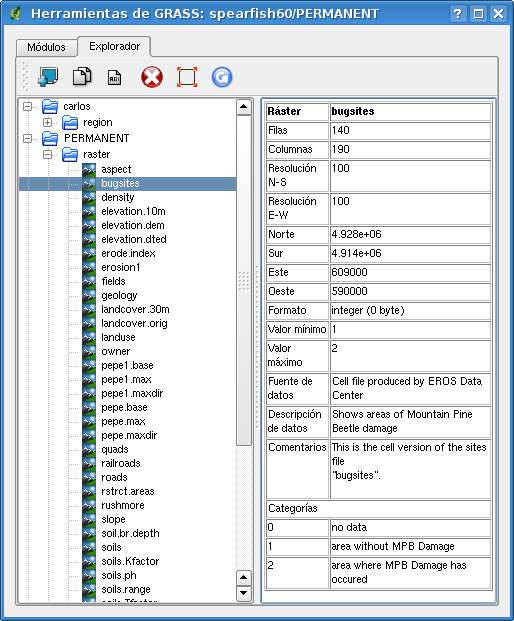
\includegraphics[clip=true, width=0.4\textwidth]{grassbrowser}}\goodgap
%   \subfigure[GRASS shell inside the toolbox]{\label{subfig:grass_shell}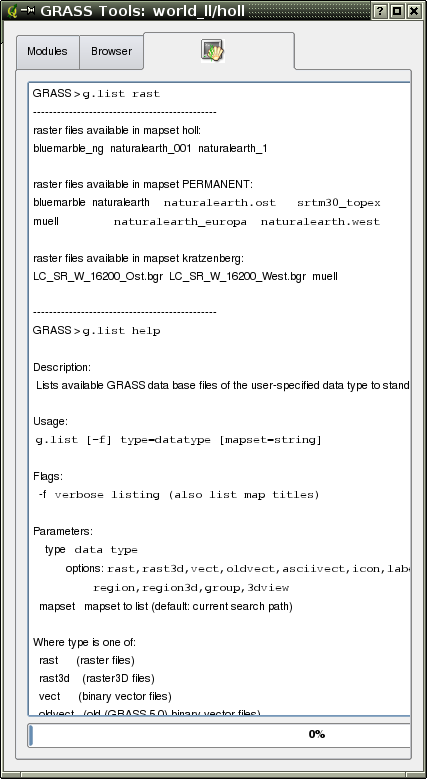
\includegraphics[clip=true, width=0.4\textwidth]{grassshell}}
%\end{figure}

\subsubsection{Customizing the modules section} \index{GRASS!toolbox!customize}
\label{sec:toolbox-customizing}

Nearly all GRASS modules can be adopted to the GRASS toolbox. A XML interface is provided to parse
the very simple XML files which configure the modules inside the toolbox.

% TODO: migrating the content of this wiki-page into the manual?
A brief description of adding new modules, changing the modules group, etc. can be found on the QGIS wiki
at \url{http://wiki.qgis.org/qgiswiki/Adding\_New\_Tools\_to\_the\_GRASS\_Toolbox}.

A sample XML file for generating the module \usertext{v.buffer} (v.buffer.qgm) looks like this:
\begin{verbatim}
<?xml version="1.0" encoding="UTF-8"?>
<!DOCTYPE qgisgrassmodule SYSTEM "http://mrcc.com/qgisgrassmodule.dtd">

<qgisgrassmodule label="Vector buffer" module="v.buffer">
        <option key="input" typeoption="type" layeroption="layer" />
        <option key="buffer"/>
        <option key="output" />
</qgisgrassmodule>
\end{verbatim}

%\begin{figure}[ht]
%\centering
%\caption{Module generated through parsing the XML-file}\label{fig:buffer-module}
%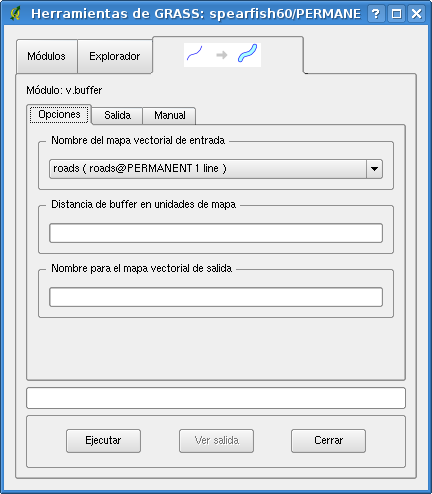
\includegraphics[clip=true, width=0.45\textwidth]{vbuffer}
%\end{figure}

The parser reads this definition and creates a new tab inside the toolbox when you select 
the module:


\subsection{Creating a new GRASS layer}\label{sec:creating_new_grass_vectors}\index{GRASS!Creating new vectors|see{editing!creating a new layer}}

With this version of QGIS it is also possible to create new vectors from within GRASS very
easily.

Just select \mainmenuopt{Plugins} > \dropmenuopt{GRASS} > 
\dropmenuopttwo{grass_new_vector_layer}{Create new GRASS layer} from the toolbar, give a new name in the text box and start digitizing.
If you encounter a greyed-out button, make sure you have a working mapset enabled. If you forgot
how to enable a mapset have a look at Section \ref{sec:load_grassdata}.

Since GRASS is able to organize all sort of geometries in one layer, there is no need to select
the geometry. This only applies to shapefile creation (see sec. \ref{sec:create shape}).

Some hints to make your digitizing more useful:
\begin{itemize}
\item Make sure to create an attribute table with its needed columns before you start digitizing
if you would like to assign attributes to your digitized object. 
Go to the table tab inside the digitize window.
\item If you plan to create a polygon layer, consider setting the mode to \usertext{No category}. 
Then start digitizing the boundaries which actually do not need an entry in the attribute table. 
If you have done this, change back to \usertext{Next not used} and start digitizing the centroids, which 
hold the attribute information of a polygon.

\end{itemize}

%\section{The GRASS Toolbar}
%The GRASS toolbar is displayed when the GRASS plugin is loaded using the
% Plugin Manager (see Section \ref{sec:managing_plugins}, \textsl{Managing
% Plugins}). Figure  shows the toolbar with each function annotated.
